\documentclass[runningheads]{llncs}
\usepackage[T1]{fontenc}
\usepackage{amsmath,amssymb}
\usepackage{graphicx}
\usepackage{booktabs}
\usepackage{array}
\usepackage{microtype}
\usepackage{tikz}

\renewcommand{\topfraction}{.9}\renewcommand{\bottomfraction}{.8}\renewcommand{\textfraction}{.08}\renewcommand{\floatpagefraction}{.75}
\usetikzlibrary{arrows.meta,positioning,fit,backgrounds}
\newcommand{\bfivezerothreeerrfivezerothreefixed}{2}
\newcommand{\bfivezerothreeerrfivezerothreelegacy}{160}
\newcommand{\bfivezerothreehealthyfixed}{40}
\newcommand{\bfivezerothreemederrfivezerothreefixed}{0.002}
\newcommand{\bfivezerothreemederrfivezerothreelegacy}{0.302}
\newcommand{\bfivezerothreemedhealthyfixed}{0.134}
\newcommand{\efivehangBnew}{24.72}
\newcommand{\efivehangBnewhttp}{80}
\newcommand{\efivehangBnewtot}{494.9}
\newcommand{\efivehangBold}{24.71}
\newcommand{\efivehangBoldhttp}{80}
\newcommand{\efivehangBoldtot}{494.7}
\newcommand{\efivehangSPonetwozeronew}{6.18}
\newcommand{\efivehangSPonetwozeronewhttp}{25}
\newcommand{\efivehangSPonetwozeronewtot}{154.7}
\newcommand{\efivehangSPonetwozeroold}{6.18}
\newcommand{\efivehangSPonetwozerooldhttp}{25}
\newcommand{\efivehangSPonetwozerooldtot}{154.6}
\newcommand{\efivehangSPthreezeronew}{3.09}
\newcommand{\efivehangSPthreezeronewhttp}{13}
\newcommand{\efivehangSPthreezeronewtot}{80.5}
\newcommand{\efivehangSPthreezeroold}{3.09}
\newcommand{\efivehangSPthreezerooldhttp}{13}
\newcommand{\efivehangSPthreezerooldtot}{80.4}
\newcommand{\efivehangSPsixzeronew}{6.20}
\newcommand{\efivehangSPsixzeronewhttp}{25}
\newcommand{\efivehangSPsixzeronewtot}{154.8}
\newcommand{\efivehangSPsixzeroold}{6.18}
\newcommand{\efivehangSPsixzerooldhttp}{25}
\newcommand{\efivehangSPsixzerooldtot}{154.5}
\newcommand{\efiveokSPsixzeronew}{0.14}
\newcommand{\efiveokSPsixzeronewhttp}{40}
\newcommand{\efiveokSPsixzeronewtot}{3.4}
\newcommand{\efiveokSPsixzeroold}{0.13}
\newcommand{\efiveokSPsixzerooldhttp}{40}
\newcommand{\efiveokSPsixzerooldtot}{2.9}
\newcommand{\efiverecoverSPsixzeronew}{0.19}
\newcommand{\efiverecoverSPsixzeronewhttp}{35}
\newcommand{\efiverecoverSPsixzeronewtot}{58.1}
\newcommand{\efiverecoverSPsixzeroold}{0.15}
\newcommand{\efiverecoverSPsixzerooldhttp}{35}
\newcommand{\efiverecoverSPsixzerooldtot}{57.5}
\newcommand{\efiverefuseSPsixzeronew}{0.18}
\newcommand{\efiverefuseSPsixzeronewhttp}{25}
\newcommand{\efiverefuseSPsixzeronewtot}{4.7}
\newcommand{\efiverefuseSPsixzeroold}{0.17}
\newcommand{\efiverefuseSPsixzerooldhttp}{25}
\newcommand{\efiverefuseSPsixzerooldtot}{4.3}
\newcommand{\phagrci}{[$-$0.284,$-$0.170]}
\newcommand{\phagrmean}{$-$0.226}
\newcommand{\phagrsame}{8}
\newcommand{\phchgci}{[$-$4.50,$-$0.24]}
\newcommand{\phchgmean}{$-$2.67}
\newcommand{\phchgsame}{7}
\newcommand{\phfuci}{[+0.00,+1.76]}
\newcommand{\phfumean}{+0.59}
\newcommand{\phfusame}{1}
\newcommand{\phrevci}{[$-$3.12,$-$0.27]}
\newcommand{\phrevmean}{$-$1.88}
\newcommand{\phrevsame}{7}
\newcommand{\predAone}{supported}
\newcommand{\predAonezero}{contradicted}
\newcommand{\predAtwo}{supported}
\newcommand{\predAthree}{supported}
\newcommand{\predAfour}{supported}
\newcommand{\predAfive}{supported}
\newcommand{\predAsix}{supported}
\newcommand{\predAseven}{supported}
\newcommand{\predAeight}{supported}
\newcommand{\predAnine}{contradicted}
\newcommand{\predBone}{supported}
\newcommand{\predBtwo}{supported}
\newcommand{\predBthree}{supported}
\newcommand{\predBfour}{supported}
\newcommand{\predBfive}{supported}
\newcommand{\predBsix}{contradicted}
\newcommand{\scRecEight}{928}
\newcommand{\scRecSeven}{312}
\newcommand{\scRemEight}{1{,}300}
\newcommand{\scSteady}{1{,}274}
\newcommand{\scStretch}{0}
\newcommand{\scTotal}{3{,}814}
\newcommand{\xaBzeroHigh}{2.056}
\newcommand{\xaBzeroMed}{0.546}
\newcommand{\xaMoneHigh}{4.411}
\newcommand{\xaMoneMed}{1.589}
\newcommand{\xaN}{160}
\newcommand{\xcsupported}{5}
\newcommand{\xctauzeroagr}{0.014}
\newcommand{\xctauzerochg}{2.225}
\newcommand{\xctaufiveagr}{0.400}
\newcommand{\xctaufivechg}{12.450}
\newcommand{\xctausixagr}{0.400}
\newcommand{\xctausixchg}{12.450}
\newcommand{\xctausevenagr}{0.400}
\newcommand{\xctausevenchg}{12.450}
\newcommand{\xctaueightagr}{0.404}
\newcommand{\xctaueightchg}{12.450}
\newcommand{\xctaunineagr}{0.626}
\newcommand{\xctauninechg}{15.119}
\newcommand{\xdOverlap}{17}
\newcommand{\xdPlaceholder}{64}
\newcommand{\xeEoneDiff}{0}
\newcommand{\xeEoneIdentical}{yes}
\newcommand{\xeEoneRows}{752}

\emergencystretch=2em
\begin{document}

\title{Specialization and Coordination in a Multi-Agent Technical Interview System: Trajectory Dynamics and Architectural Trade-offs}
\titlerunning{Specialization and Coordination in a Multi-Agent Interview System}
\author{Anonymous Author(s)}
\authorrunning{Anonymous}
\institute{Anonymous Institution}
\maketitle

\begin{abstract}
Educational and conversational systems that combine automated evaluation, language models, and reinforcement-learning controllers are frequently labelled multi-agent, even when a single monolithic controller invokes components procedurally. We investigate whether decomposing pedagogical decision-making into specialized, stateful agents with a coordination layer yields measurable behavioral, trajectory, or decision-making differences over a single-controller baseline. We extend an orchestrated technical-interview preparation system with two bounded-authority agents: a Strategy Agent managing a persistent weakness ledger across turns (proposing difficulty transitions and follow-up probes) and a Coaching Agent managing a coaching history ledger (proposing feedback depth, hints, and instructional emphasis), coordinated via unidirectional peer messaging and threshold-gated arbitration. Evaluating across 160 deterministic replay sessions (a fixed set of 64 technical-interview replay instances across 20 question orders; no live language model ran), we find that stateful coordination alters difficulty trajectories in all 160 sessions relative to the frozen single-policy PPO baseline, smoothing level changes ($15.12 \to 12.45$; cluster-bootstrap 95\% CI $[-4.50, -0.24]$) and reversals ($11.74 \to 9.87$; cluster CI $[-3.12, -0.27]$), while reducing PPO agreement ($1.000 \to 0.774$) and introducing $+0.59$ probe turns driven specifically by one replay cluster ($k=1$). However, under the tested deterministic replay configuration, the split and unified architectures produced identical decision trajectories ($\mathbb{P}(\text{agree}) = 1.0$, $1{,}280/1{,}280$ turns), indicating that architectural decomposition alone did not alter the implemented decision policy. The results indicate that, under the tested configuration, specialization primarily manifests as an architectural decomposition rather than a change in the resulting decision policy, introducing measurable end-to-end orchestration overhead ($+1.04$\,ms median per-turn latency; $0.0092$\,ms vs $0.0038$\,ms in a serialization micro-benchmark) alongside architectural characteristics such as decoupled state ledgers and isolated decision records. Threshold sensitivity experiments ($\tau \in [0.0, 0.9]$) isolate the confidence threshold as the critical gating mechanism preventing oscillation collapse. We make no claims of human candidate learning or live model performance.
\keywords{multi-agent coordination \and agent specialization \and decision-making \and trajectory dynamics \and interview practice \and arbitration}
\end{abstract}

\section{Introduction}\label{sec:intro}
Interactive educational systems that combine automated scoring, language models, and reinforcement-learning (RL) policies are increasingly described as multi-agent systems~\cite{autogen,metagpt}, even when a single monolithic controller executes every component in a fixed procedural pipeline. Whether the multi-agent label reflects a genuine scientific distinction depends on how authority and state are distributed~\cite{wj95}. If components operate as specialized autonomous agents, critical questions arise regarding coordination, decision consistency, and architectural necessity: how do specialized agents coordinate their recommendations, how does their interaction affect session trajectories, and does partitioning responsibilities across specialized agents provide measurable value over a unified controller?

We investigate these questions within an orchestrated spoken technical-interview preparation system whose deployed architecture we audit rather than assume. In its baseline configuration, the system executes an automated interview workflow driven by a single learned policy (a frozen Proximal Policy Optimization controller~\cite{ppo,sb3}) operating over a 6-dimensional state vector without concept memory. Every other pedagogical choice is governed by static threshold rules in the central hub. We extend this system by introducing two specialized, stateful agents behind a feature flag, leaving the underlying evaluator, frozen PPO policy, and candidate contract intact:
\begin{enumerate}
\item \textbf{Strategy Agent:} Maintains a private weakness ledger across turns, tracking persistent conceptual deficiencies and score trajectories to propose dynamic difficulty transitions and proactive follow-up probes.
\item \textbf{Coaching Agent:} Maintains a private coaching history ledger, tracking previously delivered hints and examples to propose feedback depth, instructional emphasis, and targeted remediation tags.
\end{enumerate}
The agents possess strictly bounded authority: they only \emph{propose}. A deterministic coordinator validates all proposals against formal schemas and authority matrices, an arbitrator resolves competing recommendations against safety bounds and the PPO policy, and the central hub remains the sole system of record. Crucially, the Strategy Agent communicates pedagogical intent to the Coaching Agent via unidirectional peer messaging, enabling aligned instructional guidance without coupling private state ledgers.

This architecture enables a rigorous empirical evaluation of multi-agent coordination and specialization. Rather than evaluating generic agent reliability or treating multi-agent design as an axiomatic virtue, we formulate three precise research questions:
\begin{description}
\item[RQ1 (Coordination and intervention dynamics):] How does stateful coordination between the Strategy and Coaching agents affect the decisions and session trajectories of the interview preparation system, compared with the frozen single-policy baseline ($B_0$)?
\item[RQ2 (Empirical effects of agent specialization):] Does separating Strategy and Coaching into distinct specialized agents yield measurable decision divergence or operational trade-offs compared to a unified technical coaching agent operating on equivalent information and tasks?
\item[RQ3 (Coordination mechanisms):] Which implemented coordination components---stateful memory, peer messaging, confidence threshold gating, or PPO interaction---are responsible for observable differences in system decisions?
\end{description}

\noindent\textbf{Summary of Findings and Contributions.}
\begin{itemize}
\item \emph{Coordination Dynamics (RQ1):} In deterministic replay across 160 sessions (operating on a fixed set of 64 technical-interview replay instances across 20 question permutation orders), stateful coordination alters difficulty trajectories in all 160 sessions relative to the frozen baseline. The Strategy Agent smooths trajectory oscillations, reducing mean level changes from 15.12 to 12.45 per session ($-2.67$, cluster-bootstrap 95\% CI \phchgci{}) and mean reversals from 11.74 to 9.87 ($-1.88$, cluster CI \phrevci{}). Agreement with the uncoordinated PPO action decreases from 1.000 to 0.774 ($-0.226$, cluster CI \phagrci{}). Proactive probes introduce an average of $+0.59$ additional turns per session (cluster CI \phfuci{}). However, a cluster sensitivity analysis reveals that this probing increase is driven entirely by a single replay cluster ($k=1$); omitting cluster 1 yields $\Delta = +0.00$ extra turns.
\item \emph{Limits of Specialization (RQ2):} Under the tested deterministic replay configuration, the split and unified architectures produced identical decisions and difficulty trajectories across all 160 sessions (1,280 turns; $\mathbb{P}(\text{agree}) = 1.0$), demonstrating that architectural decomposition alone did not alter the implemented decision policy. Ablating the Coaching Agent ($M_3$) reproduces the full two-agent system's difficulty trajectory in 160 of 160 sessions, as difficulty adaptation is structurally independent of coaching state. Specialization introduces measurable end-to-end orchestration overhead ($+1.04$\,ms median turn latency, 47.7 agent calls per session) alongside micro-benchmark serialization costs ($+0.0054$\,ms per turn; $0.0092$\,ms vs $0.0038$\,ms). Under the tested configuration, specialization primarily manifests as an architectural decomposition rather than a change in the resulting decision policy, establishing distinct state ledgers and isolated decision records rather than measured algorithmic gains.
\item \emph{Mechanism Decomposition (RQ3):} Through controlled ablations and a multi-level threshold sweep ($\tau \in [0.0, 0.9]$), we isolate the confidence threshold as the critical gating mechanism. Setting $\tau = 0.0$ collapses level changes to 2.225 and PPO agreement to 0.014, identical to removing arbitration entirely ($M_4$). Peer messaging ($M_5$) alters coaching depth and tone without destabilizing difficulty. Disabling PPO ($M_7$) alters trajectories in only 4 of 160 sessions (2.5\%), contradicting the registered prediction of $\ge 50\%$ divergence and revealing strong alignment between the Strategy Agent heuristic and the baseline rule fallback.
\end{itemize}

\noindent\textbf{What Kind of Contribution This Is.} The specialized agents, typed contracts, and authority matrix constitute \emph{architecture}; the peer messaging and threshold gating constitute \emph{coordination mechanisms}; the replay ablations and cluster-bootstrap evaluations provide \emph{empirical evidence on coordination and the limits of specialization}.

\noindent\textbf{Explicit Disclaimers.} All replay experiments execute deterministically with recorded evaluator outputs (`EVALUATOR\_MOCK\_MODE=1`); no live large language model was invoked during replay. We make \textbf{no claims} regarding candidate learning, pedagogical efficacy, interview placement success, or LLM hallucination rates. Fewer trajectory reversals reflect behavioral stability, not proven pedagogical superiority.

\section{Related Work}\label{sec:related}

Research on multi-agent systems has established several ways of distributing complex decision processes across interacting components. Classical agent-oriented work emphasizes autonomy, reactivity, pro-activeness, and social interaction as fundamental properties of agents ~\cite{wj95}. More recent LLM-based systems operationalize these ideas through structured collaboration. AutoGen, for example, uses conversational interaction as a mechanism for coordinating multiple agents ~\cite{autogen}, while MetaGPT organizes agents around specialized roles and standardized workflows ~\cite{metagpt}. These approaches show that dividing responsibility can structure complex tasks, but behavior depends also on how information and intermediate decisions move between agents.

This distinction becomes important when architectural organization is evaluated empirically. Studies comparing different agent configurations have reported task-dependent rather than universally superior arrangements ~\cite{kim2026artifact,kim2026capable}. In addition, evaluations centered on final task artifacts can obscure the internal mechanism responsible for an observed difference: a change in outcome may arise from role specialization, from the information exchanged between agents, or from the coordination procedure that determines how their outputs are combined. Recent analyses of multi-agent systems have similarly identified failures involving specification, inter-agent alignment, and verification ~\cite{mast}, indicating that the organization of interaction is itself an important part of the system being evaluated. The question is therefore not simply whether several agents can collectively solve a task, but whether the architectural separation of responsibilities changes the decisions produced when the surrounding information and decision conditions are held constant.

We treat adaptive interviewing as a sequential decision problem in which accumulated session evidence determines subsequent interactions. Reinforcement learning is one framework for mapping an observed state to actions over a sequence of decisions; our system uses PPO~\cite{ppo} as implemented in Stable-Baselines3~\cite{sb3}. In a technical interview, however, the information relevant to longitudinal assessment progression need not be identical to the information used for feedback, hints, or follow-up behavior. A centralized controller can therefore couple responsibilities that operate on different aspects of an evolving interaction. When the controller acts on a compact representation of a longer session, an individual decision also affects the state encountered at later turns, making the resulting trajectory an important object of analysis rather than merely a sequence of independent actions.

Separating assessment progression from coaching-related responsibilities may change the organization and ownership of state without changing the final decisions, whereas introducing additional decision sources can alter the trajectory through the mechanism used to admit and reconcile their proposals. The two effects are easy to conflate when decomposition and coordination are introduced simultaneously, so a controlled evaluation needs to distinguish them.

Safety-oriented reinforcement learning provides the complementary principle that adaptive decisions need not possess unrestricted authority. Shielding and supervisory approaches place external constraints around learned policies so that unsafe actions can be rejected, overridden, or restricted before they reach the environment~\cite{shield,safe}. This separation between policy generation and authoritative enforcement becomes particularly relevant when additional stateful components are introduced. A component may maintain information relevant to its role and recommend an action without being permitted to modify the authoritative state directly. Such a distinction allows proposal generation, validation, arbitration, and final commitment to be treated as separate responsibilities rather than allowing every participating component to act as a state owner.

Once several components can contribute recommendations, the system must determine which information each component owns, what authority accompanies a proposal, how proposals are reconciled with the underlying policy, and which constraints remain authoritative when they conflict. These questions require the internal decision path to be observable if their individual effects are to be separated experimentally.

The literature consequently provides the principal building blocks for distributed responsibility, sequential adaptation, and supervisory constraint enforcement, while leaving open an important empirical distinction between \textbf{coordination and specialization}. Distributed state and role separation may change the architecture without changing matched decisions, whereas coordination and arbitration may directly affect the trajectory through which decisions are produced. Authority boundaries add a further dimension by determining whether those distributed components remain subordinate to a single authoritative state owner. The present study uses this distinction as the basis for its architecture: specialized components maintain bounded private state and communicate constrained proposals, while authoritative commitment remains centralized. The architectural structure required to make those distinctions explicit is described next.

\section{System Architecture and Authority Topology}\label{sec:design}
\noindent\textbf{Reference Monolithic Workflow.}
A browser client sends a spoken answer to a backend, which transcribes it and calls an \emph{InterviewOrchestrator} (the hub; Fig.~\ref{fig:arch}). The hub owns one session-state dictionary and one lock and runs a fixed per-turn pipeline: (1) a learned \emph{evaluator} (sentence-embedding similarity $S_1$, a concept index $S_2$ and a fine-tuned cross-encoder $R$; $0.15S_1{+}0.35S_2^{\mathrm{eff}}{+}0.50R$ with a cap when a mandatory concept is missed) returns a score and concept evidence; (2) a strict hand-off contract treats a non-finite or out-of-range score as an evaluator failure and fails closed; (3) feedback is produced by a template or an optional local LLM; (4) the hub commits the turn; (5) a baseline schedule and then a frozen PPO policy~\cite{sb3,ppo} propose an easier/same/harder action, followed by a rule layer of six guardrails; (6) a threshold rule decides whether a follow-up question is injected (at most two in a row). Before this work only the PPO policy was a reactive learned decision-maker; the LLM never chose an action. All of this is unchanged when the multi-agent flag is off, and a test shows that with the flag on but no agent contributing the trajectory is identical (Sect.~\ref{sec:results}).

\noindent\textbf{Specialized Agent Roles and Private State.}
\begin{table}[tbp]
\centering\small
\caption{Authority matrix, generated from the enforcing code (\texttt{agents/multiagent/} \texttt{authority.py}). Neither agent has state-write authority; the hub commits alone.}\label{tab:authority}
\begin{tabular}{>{\raggedright\arraybackslash}p{1.5cm}>{\raggedright\arraybackslash}p{2.5cm}>{\raggedright\arraybackslash}p{2.3cm}>{\raggedright\arraybackslash}p{2.8cm}>{\raggedright\arraybackslash}p{2.0cm}}
\toprule
Agent & May propose & Private state & Cannot & On invalid output \\
\midrule
\textbf{Strategy} & difficulty\_action (Easier\slash Same\slash Harder); probe request (concept, kind); strategy mode & weakness ledger (per-concept miss counts, probe history, trend) & write or overwrite any score; set a difficulty level directly; terminate the session; edit history; override hard constraints or guardrail overrides; call another agent & invalid / stale / low-confidence / timed-out proposal is dropped; PPO proposal stands \\
\midrule
\textbf{Coaching} & feedback depth; hint / example flags; concepts to emphasise; remediation tag; tone & coaching history (hints/examples given, repeated misconceptions) & alter evaluator results or scores; cite concepts absent from the evaluator evidence; request difficulty changes; request follow-ups; terminate the session & invalid plan is dropped; the existing template feedback is used unchanged \\
\bottomrule
\end{tabular}

\end{table}
Table~\ref{tab:authority} lists what each agent may propose and may not do. Applying the principle of least privilege~\cite{ss75}, neither agent possesses state-write privileges. Both agents implement a single method \texttt{propose(observation, peer)}, receive an immutable, validated \texttt{TurnObservation} (score, evidence lists, difficulty, score history, progress, follow-up counters; counters carry the value the hub will commit), and return a typed proposal. They are rule- and ledger-based, not LLM-driven; they are the smallest design that has private persistent state, pro-active proposals and a communication channel, which are the properties of weak agency~\cite{wj95} that the existing roles lacked. We make no claim of autonomy beyond that.

\paragraph{Strategy Agent.} Objective: maintain configured difficulty adaptation while tracking persistent weaknesses within the follow-up budget. Private state: per concept, the distinct turns in which the evaluator listed it as missing or incorrect, which concepts were later covered, probes already requested, and an exponential moving average (EMA) of scores. Rules, first match wins: \emph{recover} (current score $<0.35$ and mean of the last two $<0.5$, or a weakness that survived its probes while the score stays $<0.5$) $\rightarrow$ Easier; \emph{remediate} (a concept missed on $\ge 2$ distinct turns and unresolved) $\rightarrow$ Same plus a probe request for that concept; \emph{stretch} (score $\ge0.8$, average $\ge0.7$, last three $\ge0.6$, no open weakness) $\rightarrow$ Harder; otherwise \emph{steady}. Non-\emph{steady} proposals use confidence $\min(0.95, 0.5{+}0.1n)$ for $n$ cited evidence items (a documented heuristic rather than a calibrated probability), while \emph{steady} proposals are assigned 0.45 (below the arbitration threshold $\tau = 0.6$, so the PPO action stands unless the ledger supports a change).

\paragraph{Coaching Agent.} Objective: choose how to coach after an evaluated answer. Private state: concept miss counts and the hints and examples already given. Decisions: up to two concepts to emphasize (incorrect claims first, then repeatedly missed, then evaluator order); a hint if concepts are missing, the score is $<0.6$ and fewer than two hints were given for the lead concept; an example when the lead concept was missed before and no example was given yet; depth (\emph{detailed} if score $<0.4$ or a repeated miss, \emph{brief} if $\ge0.85$ with nothing missing); tone; a remediation tag. A Strategy proposal delivered as a peer message modifies the plan (\emph{recover}: detailed and encouraging; \emph{stretch}: brief; \emph{remediate}: remediation tag on the probed concept). A deterministic renderer applies the plan to the existing feedback dictionary: it adds presentation fields and may prepend a priority tip to, or truncate, the existing improvement and communication-tip lists, and it raises if any protected evaluator field (score, grade, concept and claim lists, transcript, decision source) would change.

\noindent\textbf{Communication and State Ownership.}\label{sec:comm}
Every observation, proposal and decision is a typed object (\texttt{pydantic}, unknown fields rejected, NaN and out-of-range values rejected). The coordinator records each call as an envelope with session, turn, sender, recipient, state version and provenance, and every accept/reject/modify outcome as a decision record with a reason code. Optimistic concurrency uses a \emph{state version} that counts committed turns: a proposal whose version, turn or session differs from the observation, or from the hub's current version, is stale and dropped; a second answer from the same agent for the same version is a duplicate and dropped. The hub builds observations, commits state, increments the version, and persists agent memory in its session snapshot so that a recovered session resumes with the agents' ledgers.

\begin{figure}[tbp]
\centering
\resizebox{0.70\textwidth}{!}{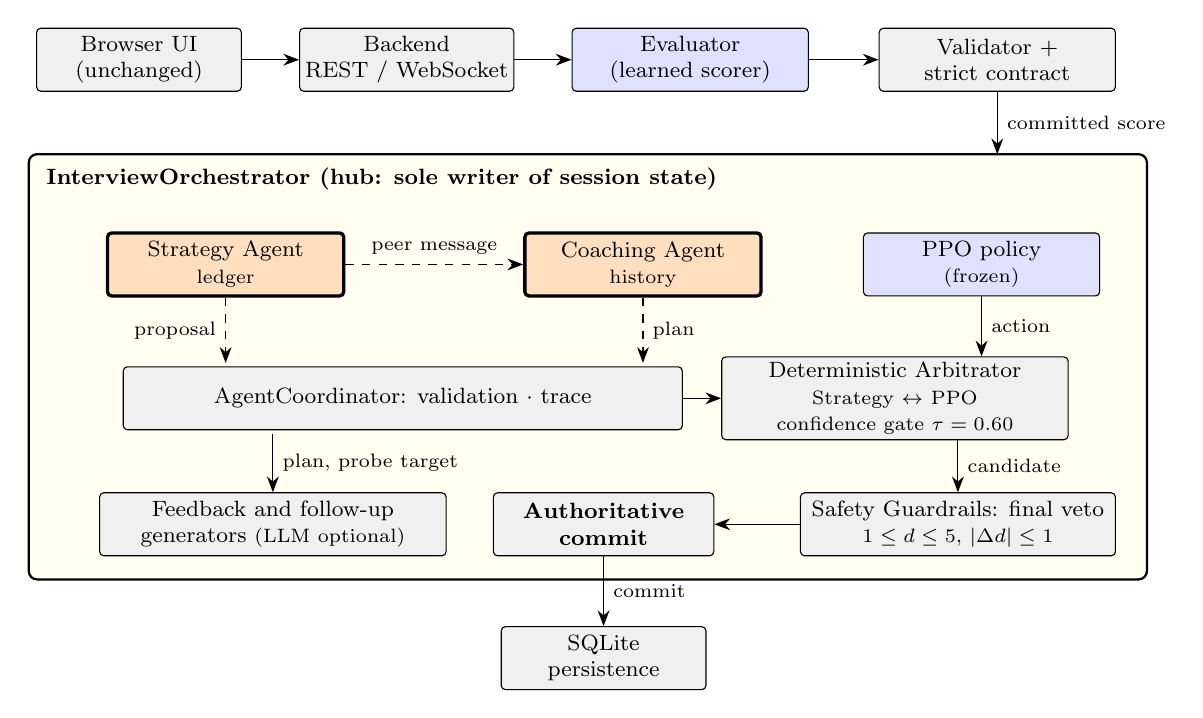
\begin{tikzpicture}[font=\footnotesize,
  box/.style={draw, rounded corners=1.5pt, minimum height=8mm, align=center, inner sep=2pt},
  det/.style={box, fill=gray!12},
  lrn/.style={box, fill=blue!12},
  agt/.style={box, fill=orange!25, very thick},
  arr/.style={-{Stealth[length=2mm]}, thin},
  darr/.style={-{Stealth[length=2mm]}, thin, dashed}]
% outside the hub
\node[det, minimum width=26mm] (ui) at (0.5,6.2) {Browser UI\\(unchanged)};
\node[det, minimum width=26mm] (be) at (3.9,6.2) {Backend\\REST / WebSocket};
\node[lrn, minimum width=30mm] (ev) at (7.5,6.2) {Evaluator\\(learned scorer)};
\node[det, minimum width=30mm] (val) at (11.4,6.2) {Validator +\\strict contract};
\draw[arr] (ui) -- (be); \draw[arr] (be) -- (ev); \draw[arr] (ev) -- (val);
% hub
\draw[rounded corners=3pt, thick, fill=yellow!6] (-0.9,-0.4) rectangle (13.3,5.0);
\node[anchor=north west, font=\footnotesize\bfseries] at (-0.8,4.95) {InterviewOrchestrator (hub: sole writer of session state)};
\node[agt, minimum width=30mm] (st) at (1.6,3.6) {Strategy Agent\\{\scriptsize ledger}};
\node[agt, minimum width=30mm] (co) at (6.9,3.6) {Coaching Agent\\{\scriptsize history}};
\node[lrn, minimum width=30mm] (pp) at (11.2,3.6) {PPO policy\\{\scriptsize (frozen)}};
\node[det, minimum width=71mm] (cd) at (3.85,1.9) {AgentCoordinator: validation $\cdot$ trace};
\node[det, minimum width=44mm] (ar) at (10.1,1.9) {Deterministic Arbitrator\\{\scriptsize Strategy $\leftrightarrow$ PPO}\\{\scriptsize confidence gate $\tau = 0.60$}};
\node[det, minimum width=40mm] (gr) at (10.9,0.3) {Safety Guardrails: final veto\\{\scriptsize $1 \le d \le 5$, $|\Delta d| \le 1$}};
\node[det, minimum width=44mm] (fb) at (2.2,0.3) {Feedback and follow-up\\generators {\scriptsize (LLM optional)}};
\node[det, minimum width=28mm] (cm) at (6.4,0.3) {\textbf{Authoritative}\\\textbf{commit}};
\node[det, minimum width=26mm] (db) at (6.4,-1.4) {SQLite\\persistence};
\draw[arr] (val.south) -- node[right]{\scriptsize committed score} (11.4,5.0);
\draw[darr] (st) -- node[above]{\scriptsize peer message} (co);
\draw[darr] (st.south) -- node[left]{\scriptsize proposal} (1.6,2.35);
\draw[darr] (co.south) -- node[right]{\scriptsize plan} (6.9,2.35);
\draw[arr] (pp.south) -- node[right]{\scriptsize action} (pp.south |- ar.north);
\draw[arr] (cd.east) -- (ar.west);
\draw[arr] (ar.south -| gr.north) -- node[right]{\scriptsize candidate} (gr.north);
\draw[arr] (gr.west) -- (cm.east);
\draw[arr] (2.2,1.45) -- node[right]{\scriptsize plan, probe target} (fb.north);
\draw[arr] (cm.south) -- node[right]{\scriptsize commit} (db.north);
\end{tikzpicture}
}
\caption{System architecture and authority topology of the bounded multi-agent configuration. The \texttt{InterviewOrchestrator} retains sole authority over committed session state. Strategy and Coaching maintain separate private ledgers and contribute proposal-only outputs. Strategy may transmit a unidirectional operational mode to Coaching, while both components submit typed proposals to the coordinator. The PPO policy independently provides the baseline difficulty action. The coordinator routes eligible proposals to deterministic arbitration, after which downstream guardrails retain final veto authority before the hub commits the resulting state transition.}\label{fig:arch}
\end{figure}

\section{Orchestration, Arbitration and Validation}\label{sec:arbitration}
\begin{figure}[tbp]
\centering
\resizebox{0.68\textwidth}{!}{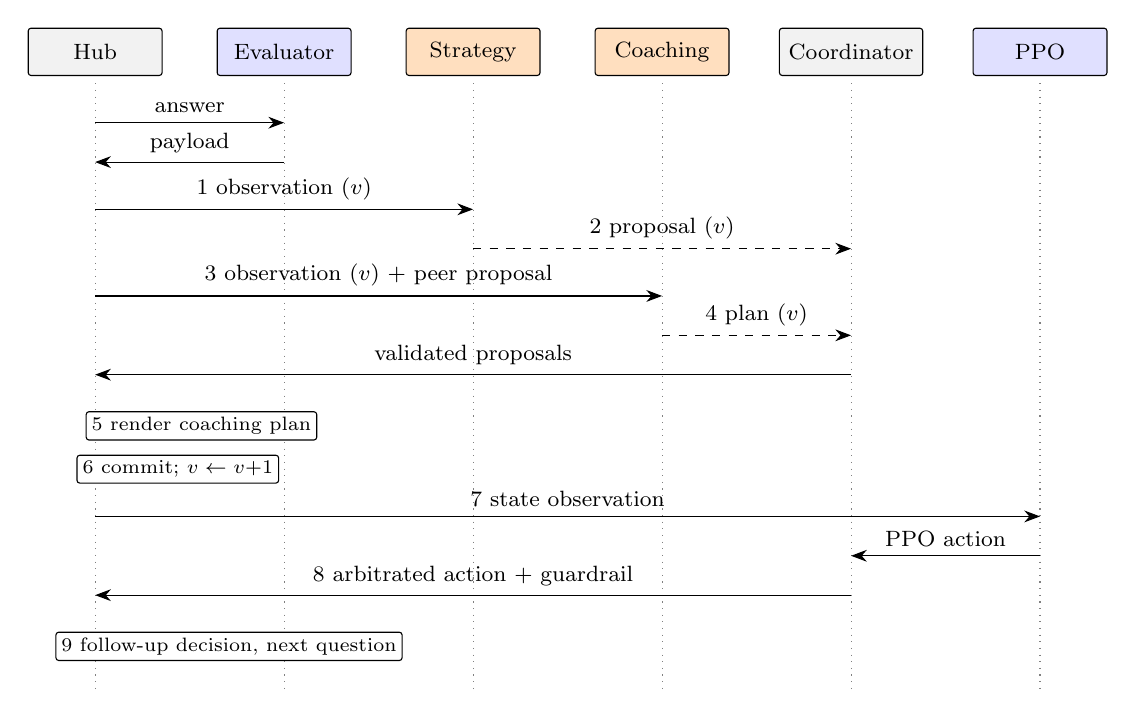
\begin{tikzpicture}[font=\footnotesize, x=1cm, y=1cm,
  life/.style={draw, rounded corners=1pt, minimum width=17mm, minimum height=6mm, align=center, fill=gray!10},
  msg/.style={-{Stealth[length=2mm]}, thin},
  dmsg/.style={-{Stealth[length=2mm]}, thin, dashed},
  note/.style={draw, fill=white, rounded corners=1pt, inner sep=2pt, font=\scriptsize}]
\def\xh{0} \def\xe{2.4} \def\xs{4.8} \def\xc{7.2} \def\xd{9.6} \def\xp{12}
\node[life] (hub) at (\xh,0) {Hub};
\node[life, fill=blue!12] (ev) at (\xe,0) {Evaluator};
\node[life, fill=orange!25] (st) at (\xs,0) {Strategy};
\node[life, fill=orange!25] (co) at (\xc,0) {Coaching};
\node[life] (cd) at (\xd,0) {Coordinator};
\node[life, fill=blue!12] (pp) at (\xp,0) {PPO};
\foreach \x in {\xh,\xe,\xs,\xc,\xd,\xp} \draw[gray, dotted] (\x,-0.4) -- (\x,-8.1);
\draw[msg] (\xh,-0.9) -- node[above]{answer} (\xe,-0.9);
\draw[msg] (\xe,-1.4) -- node[above]{payload} (\xh,-1.4);
\draw[msg] (\xh,-2.0) -- node[above]{1 observation $(v)$} (\xs,-2.0);
\draw[dmsg] (\xs,-2.5) -- node[above]{2 proposal $(v)$} (\xd,-2.5);
\draw[msg] (\xh,-3.1) -- node[above]{3 observation $(v)$ + peer proposal} (\xc,-3.1);
\draw[dmsg] (\xc,-3.6) -- node[above]{4 plan $(v)$} (\xd,-3.6);
\draw[msg] (\xd,-4.1) -- node[above]{validated proposals} (\xh,-4.1);
\node[note] at (\xh+1.35,-4.75) {5 render coaching plan};
\node[note] at (\xh+1.05,-5.3) {6 commit; $v \leftarrow v{+}1$};
\draw[msg] (\xh,-5.9) -- node[above]{7 state observation} (\xp,-5.9);
\draw[msg] (\xp,-6.4) -- node[above]{PPO action} (\xd,-6.4);
\draw[msg] (\xd,-6.9) -- node[above]{8 arbitrated action + guardrail} (\xh,-6.9);
\node[note] at (\xh+1.7,-7.55) {9 follow-up decision, next question};
\end{tikzpicture}
}
\caption{One interview turn as implemented (verbal path). Steps 1--4 happen before the hub commits; arbitration (8) follows the PPO suggestion. On the code-submission path only the Strategy proposal is collected.}\label{fig:flow}
\end{figure}
Figure~\ref{fig:flow} shows one turn. \textbf{Difficulty precedence} (deterministic code, evaluated by ablation rather than assumed optimal): (1) hard constraints (infrastructure failure forces Same; levels stay in $[1,5]$); (2) the guardrail layer, applied last to whichever candidate was selected, wins whenever a rule fires (G3 and G6 hold or raise difficulty, so this layer does not act solely in a downward direction); (3) a validated Strategy proposal with confidence $c \ge \tau$ and cited evidence supersedes the PPO action, recorded as a \emph{conflict}; (4) the PPO action, or the labeled non-RL heuristic when PPO is unavailable. A proposal that cannot take effect at the bounds is recorded as \emph{modified}. \textbf{Probe precedence:} the hard cap of two consecutive follow-ups, then a Strategy probe whose concept appeared in the evaluator's evidence earlier in this session and whose confidence satisfies $c \ge \tau$ (it may add a probe the thresholds would not trigger, or retarget the default one), then the hub's original threshold rule. The retargeted concept is passed to the template follow-up generator; the LLM prompt is not changed.

\textbf{PPO integration.} PPO keeps its role and its 6-D state and 3-action definitions; the reference policy was trained once with a fixed configuration and seed (seed 123, 100,000 nominal training steps) and then frozen before the multi-agent evaluation; no hyperparameter search or result-based checkpoint selection was performed. Its action is one input to arbitration. The agents never see the PPO action before they propose, and the paper makes no claim that the agents improve PPO. Calling this multi-agent RL would be wrong: one policy is learned, and the agents are not trained.

\textbf{Guardrails.} The deployed hub uses an inline copy of the rule layer that differs from the module used by the training environment. A configuration key selects \texttt{legacy\_inline} (default; deployed behavior) or \texttt{canonical}; both are reported separately. On a synthetic grid (39,930 points, hesitation $\mathit{hes}=1-\mathit{conf}$, with $\mathit{conf}$ the acoustic confidence) the two disagree on 4,728 points (11.8\%) in G2, G6 and the no-override case; this is a property of the grid, not a deployment frequency, and a regression test pins it.

\begin{figure}[tbp]
\centering
\resizebox{0.68\textwidth}{!}{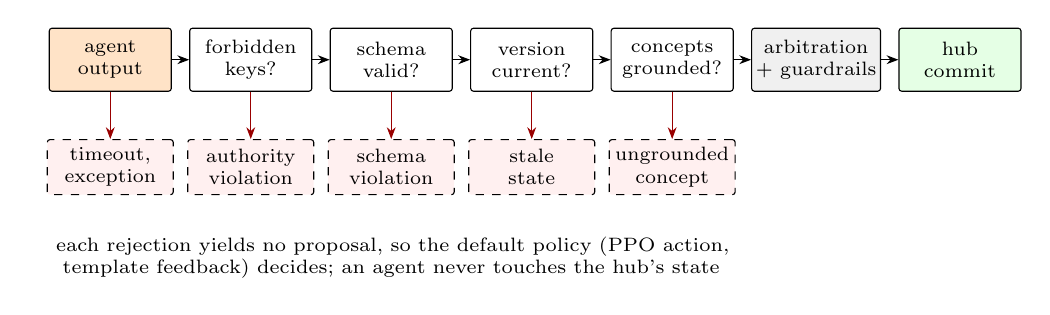
\begin{tikzpicture}[font=\scriptsize, node distance=2.2mm,
  s/.style={draw, rounded corners=1pt, minimum height=8mm, minimum width=15.5mm, align=center, inner sep=1.5pt},
  r/.style={draw, dashed, rounded corners=1pt, minimum height=7mm, minimum width=16mm, align=center, fill=red!6, inner sep=1.5pt},
  arr/.style={-{Stealth[length=1.5mm]}, thin}]
\node[s, fill=orange!22] (raw) {agent\\output};
\node[s, right=of raw] (au) {forbidden\\keys?};
\node[s, right=of au] (sc) {schema\\valid?};
\node[s, right=of sc] (sv) {version\\current?};
\node[s, right=of sv] (gr) {concepts\\grounded?};
\node[s, right=of gr, fill=gray!12] (ar) {arbitration\\+ guardrails};
\node[s, right=of ar, fill=green!10] (cm) {hub\\commit};
\foreach \a/\b in {raw/au,au/sc,sc/sv,sv/gr,gr/ar,ar/cm} \draw[arr] (\a) -- (\b);
\node[r, below=6mm of raw] (f0) {timeout,\\exception};
\node[r, below=6mm of au] (f1) {authority\\violation};
\node[r, below=6mm of sc] (f2) {schema\\violation};
\node[r, below=6mm of sv] (f3) {stale\\state};
\node[r, below=6mm of gr] (f4) {ungrounded\\concept};
\foreach \a/\b in {raw/f0,au/f1,sc/f2,sv/f3,gr/f4} \draw[arr, red!60!black] (\a) -- (\b);
\node[below=4mm of f2, text width=9cm, align=center] {each rejection yields no proposal, so the default policy (PPO action, template feedback) decides; an agent never touches the hub's state};
\end{tikzpicture}
}
\caption{Validation pipeline every proposal passes before arbitration. Each rejection yields no proposal; the default policy decides.}\label{fig:valid}
\end{figure}
\paragraph{Proposal Validation.} Before any proposal reaches arbitration, the coordinator executes four sequential checks (Fig.~\ref{fig:valid}): (1)~strict Pydantic schema validation (\texttt{extra=forbid}, NaN and out-of-range rejection); (2)~recursive scanning against the 18 forbidden state keys; (3)~optimistic concurrency verification matching the hub's current committed turn version; and (4)~concept evidence grounding. If an agent raises an unhandled exception or exceeds the configured timeout (150\,ms), its proposal is dropped and the hub proceeds with the default policy.

\section{Experimental Methodology}\label{sec:method}

\subsection{Evaluation Environment and Replay Dataset}
To rigorously evaluate coordination and specialization without confounding stochastic variance from external API calls, all experiments are conducted via deterministic replay through the real orchestrator hub with \texttt{EVALUATOR\_MOCK\_MODE=1}.

\noindent\textbf{Replay Stimuli and Dataset Structure.} All experiments operate on a fixed set of 64 technical-interview replay instances. Each instance provides a deterministic sequence of evaluator inputs, enabling matched comparisons across the split and unified architectures and their ablations. The 64 instances cover 8 technical interview question domains (arrays, dynamic programming, trees/graphs, system design, concurrency, databases, networking, and object-oriented design), with 8 candidate answers per domain evaluated against rubric keywords, fine-tuned cross-encoders, and concept extractors. In replay mode, the hub consumes these fixed evaluator inputs directly, driving the full orchestrator state machine and agent coordinator. Follow-up probe questions receive the candidate payload corresponding to the root concept.

\noindent\textbf{The 8-Cluster Structure.} A critical methodological detail is that replay sessions are generated by combining the 8 underlying replay clusters with 20 seeded pseudo-random question-order permutations (seeds 42--61), yielding $N = 160$ sessions per experimental condition. These 160 sessions are \textbf{not independent samples}; they reuse the identical 8 replay clusters. Presenting order permutations as independent evaluation sessions would artificially deflate variance and produce overconfident inferences. We therefore explicitly model the 8 underlying replay clusters as the independent structural units in all statistical analyses.

\noindent\textbf{Evaluation Mode.} All experimental evidence is generated via deterministic replay through the real orchestrator hub, testing coordination and trajectory dynamics under fixed stimuli. No live generative LLM is invoked; the LLM gateway is stubbed as down, and deterministic template renderers handle text output, ensuring that trajectory differences are attributable solely to the evaluated coordination and agent architectures.

\subsection{Baseline and Ablation Matrix}
To address RQ1 (coordination dynamics) and RQ3 (coordination mechanisms), we evaluate the baseline platform alongside controlled ablation conditions across the identical 160 replay sessions:
\begin{itemize}
\item \textbf{Frozen Baseline ($B_0$):} The original single-controller workflow without agents. Difficulty transitions are chosen solely by the frozen PPO policy (or rule fallback) bounded by guardrails; follow-up probes are governed by the static hub threshold.
\item \textbf{Full Multi-Agent System ($M_1$):} The complete coordinated architecture with Strategy Agent, Coaching Agent, peer messaging, authority enforcement, and threshold-gated arbitration ($\tau = 0.6$).
\item \textbf{Silent Agent ($M_2$):} The multi-agent layer is active, but agents emit zero proposals, testing whether the coordination infrastructure is completely transparent when silent.
\item \textbf{Coaching Ablated ($M_3$):} The Coaching Agent is disabled while Strategy remains active, testing whether difficulty trajectories are independent of coaching state.
\item \textbf{Arbitration Ablated ($M_4$):} Arbitration checks (confidence threshold, evidence requirement, one-step bound) are removed, admitting raw Strategy proposals.
\item \textbf{Peer Messaging Ablated ($M_5$):} Strategy proposals are not delivered to Coaching as peer messages, isolating the effect of inter-agent information exchange.
\item \textbf{PPO Policy Ablated ($M_7$):} The learned PPO policy is disabled, falling back to a deterministic heuristic rule to evaluate interaction between Strategy heuristics and the baseline.
\item \textbf{Canonical Guardrails ($B_{0c}$):} Baseline workflow evaluated with canonical \texttt{rl/guardrails.py} instead of deployed inline rules.
\end{itemize}

\subsection{Framework for Evaluating Agent Specialization (RQ2)}
To evaluate whether decomposing technical coaching into specialized agents provides measurable value over a unified controller (RQ2), we formulate a controlled comparative framework contrasting:
\begin{enumerate}
\item \textbf{Specialized Architecture ($M_{\text{split}}$):} The two-agent baseline ($M_1$) partitioning responsibilities across Strategy and Coaching with disjoint state ledgers and explicit peer messaging.
\item \textbf{Unified Architecture ($M_{\text{unified}}$):} A monolithic agent (\texttt{UnifiedCoachAgent}) maintaining a joint session ledger and synthesizing difficulty actions, follow-up probes, and coaching plans in a single dispatch.
\end{enumerate}

\noindent\textbf{Equivalence Conditions.} To ensure a fair comparison, both configurations receive identical observation inputs, identical question sequences, identical heuristic decision thresholds, and identical arbitration rules. We evaluate five operational outcomes: (1)~decision agreement rate ($\mathbb{P}(\text{Decision}_{\text{unified}} = \text{Decision}_{\text{split}})$); (2)~difficulty trajectory divergence; (3)~follow-up probe selection; (4)~per-turn dispatch and serialization latency; and (5)~architectural state encapsulation (schema separation and ledger isolation).

\subsection{Threshold Decomposition (Experiment XC)}
Because the unarbitrated condition ($M_4$) simultaneously removes the confidence threshold, evidence verification, and one-step limits, it cannot isolate which mechanism prevents oscillation collapse. We therefore execute Experiment XC, sweeping the confidence threshold $\tau \in \{0.0, 0.5, 0.6, 0.7, 0.8, 0.9\}$ across the same 160 replay sessions while holding all other safety envelopes and evidence checks active.

\subsection{Statistical Methodology}
For session-level point estimates and paired differences, we compute standard non-parametric percentile bootstrap intervals with $B = 10{,}000$ resamples. To account for the 8-cluster dependency, we implement a cluster bootstrap over the 8 underlying replay clusters following Field and Welsh~\cite{fw07} ($B = 10{,}000$), resampling entire replay clusters with replacement. In addition, we report a leave-one-cluster-out (LOCO) sensitivity analysis to verify whether observed effects depend on individual influential replay clusters. All reported bootstrap confidence intervals are descriptive measures of parameter dispersion across resamples; no formal null-hypothesis significance tests or $p$-values are evaluated.

\section{Results}\label{sec:results}
All reported results are derived from deterministic REPLAY of recorded evaluator outputs unless explicitly noted. All sessions within a condition are dependent across question orders due to the 8-cluster structure (Sect.~\ref{sec:method}).

\noindent\textbf{Trajectory Divergence and Reduced Level Changes (RQ1).} Enabling the agent layer ($M_1$) altered the difficulty trajectory relative to the frozen baseline ($B_0$) in \textbf{all 160 replay sessions (100\%)} (A7; Table~\ref{tab:xapaired}). The $M_1$ trajectories show fewer level changes and reversals than $B_0$: mean level changes fell from 15.12 to 12.45 per session (point difference $-2.67$, naive session bootstrap 95\% CI $[-3.19, -2.13]$), and mean reversals fell from 11.74 to 9.87 per session ($-1.88$, naive CI $[-2.28, -1.46]$). Agreement with the uncoordinated PPO action dropped from 0.626 to 0.400 (point difference $-0.226$, cluster CI \phagrci{}), with Strategy proposals winning pre-guardrail arbitration in 11.9 decisions per session and remaining the final unoverridden action source in 6.669 decisions after downstream guardrail evaluation (\textbf{strat.} in Table~\ref{tab:xa}).


\begin{table}[tbp]
\centering\scriptsize\setlength{\tabcolsep}{3pt}
\caption{Replay ablation summary across 160 sessions per condition (mean per session unless noted as counts). \textbf{compl./auth./trans.}: sessions completing, keeping committed scores authoritative, and preserving valid transitions. \textbf{chg./rev.}: mean level changes and reversals; \textbf{agr.}: fraction of decisions agreeing with the PPO action; \textbf{gfire}: guardrail overrides; \textbf{strat.}: decisions where the Strategy Agent was the final action source; \textbf{byp.}: sessions with guardrail bypass; \textbf{p50/p95}: pooled per-turn latency in ms; \textbf{calls}: agent calls per session.}\label{tab:xa}
\resizebox{\textwidth}{!}{\begin{tabular}{lcccrrrrrrrrr}
\toprule
Cond. & compl. & auth. & trans. & chg. & rev. & agr. & gfire & strat. & byp. & p50 & p95 & calls\\
\midrule
B0 & 160 & 160 & 160 & 15.119 & 11.744 & 0.626 & 9.588 & 0.0 & 0 & 0.546 & 2.056 & -- \\
B7 & 160 & 160 & 160 & 2.675 & 1.256 & -- & 3.831 & 0.0 & 0 & 0.463 & 1.059 & -- \\
B0c & 160 & 160 & 160 & 15.119 & 11.744 & 0.626 & 9.588 & 0.0 & 0 & 0.553 & 2.004 & -- \\
M1 & 160 & 160 & 160 & 12.45 & 9.869 & 0.4 & 6.838 & 6.669 & 0 & 1.589 & 4.411 & 47.68 \\
M2 & 160 & 160 & 160 & 15.119 & 11.744 & 0.626 & 9.588 & 0.0 & 0 & 1.218 & 3.513 & 23.25 \\
M3 & 160 & 160 & 160 & 12.45 & 9.869 & 0.4 & 6.838 & 6.669 & 0 & 1.118 & 3.189 & 23.84 \\
M4 & 160 & 160 & 160 & 2.225 & 1.0 & 0.014 & 0.0 & 19.619 & 3 & 1.573 & 4.357 & 47.68 \\
M5 & 160 & 160 & 160 & 12.45 & 9.869 & 0.4 & 6.838 & 6.669 & 0 & 1.581 & 4.553 & 47.68 \\
M6 & 160 & 160 & 160 & 12.45 & 9.869 & 0.4 & 6.838 & 6.669 & 0 & 1.592 & 4.46 & 47.68 \\
M8 & 160 & 160 & 160 & 12.45 & 9.869 & 0.4 & 6.838 & 6.669 & 0 & 1.575 & 4.35 & 47.68 \\
M7 & 160 & 160 & 160 & 2.706 & 1.312 & -- & 3.812 & 9.037 & 0 & 1.502 & 2.968 & 47.68 \\
M1c & 160 & 160 & 160 & 12.45 & 9.869 & 0.4 & 6.838 & 6.669 & 0 & 1.573 & 4.534 & 47.68 \\
\bottomrule
\end{tabular}
}
\end{table}

\begin{table}[tbp]
\centering\scriptsize\setlength{\tabcolsep}{3pt}
\caption{Paired differences ($A - B$) over identical 160 replay sessions: fraction of sessions with divergent difficulty paths, paired mean differences with naive session-level 95\% percentile-bootstrap intervals, and pooled median turn latency delta. Intervals are descriptive due to cluster reuse.}\label{tab:xapaired}
\resizebox{\textwidth}{!}{\begin{tabular}{lrcccc}
\toprule
A$-$B & path$\ne$ & $\Delta$ level chg. & $\Delta$ reversals & $\Delta$ PPO agree & $\Delta$ p50 ms\\
\midrule
M1$-$B0 & 1.0 & $-$2.669 [$-$3.188,$-$2.131] & $-$1.875 [$-$2.275,$-$1.462] & $-$0.226 [$-$0.244,$-$0.208] & +1.043 [+1.000,+1.079] \\
M2$-$B0 & 0.0 & 0 & 0 & 0 & +0.672 [+0.646,+0.698] \\
M3$-$M1 & 0.0 & 0 & 0 & 0 & $-$0.471 [$-$0.511,$-$0.425] \\
M4$-$M1 & 1.0 & $-$10.225 [$-$10.544,$-$9.900] & $-$8.869 [$-$9.275,$-$8.463] & $-$0.387 [$-$0.403,$-$0.370] & $-$0.016 [$-$0.065,+0.033] \\
M5$-$M1 & 0.0 & 0 & 0 & 0 & $-$0.008 [$-$0.059,+0.037] \\
M6$-$M1 & 0.0 & 0 & 0 & 0 & +0.004 [$-$0.030,+0.053] \\
M8$-$M1 & 0.0 & 0 & 0 & 0 & $-$0.013 [$-$0.057,+0.032] \\
M7$-$B7 & 0.025 & +0.031 [+0.000,+0.081] & +0.056 [+0.006,+0.125] &  & +1.039 [+0.996,+1.070] \\
B0c$-$B0 & 0.0 & 0 & 0 & 0 & +0.008 [$-$0.019,+0.027] \\
M1c$-$M1 & 0.0 & 0 & 0 & 0 & $-$0.016 [$-$0.055,+0.032] \\
\bottomrule
\end{tabular}
}
\end{table}

\noindent\textbf{Cluster Dependence, Fragility, and Proactive Probing Sensitivity.} Because the 160 sessions reuse 8 underlying replay clusters, treating sessions as independent underestimates parameter uncertainty. A post-hoc cluster bootstrap over the 8 replay clusters (Field and Welsh~\cite{fw07}, $B = 10{,}000$) yields wider, defensible intervals: level changes \phchgmean{} \phchgci{}, reversals \phrevmean{} \phrevci{}, and PPO action agreement \phagrmean{} \phagrci{}. The negative sign for level changes and reversals is shared across 7 of the 8 replay clusters.

Proactive probing added an average of \phfumean{} turns per session (naive CI $[+0.34, +0.85]$, cluster CI \phfuci{}). However, cluster-level decomposition reveals that this probe increase is present in \textbf{only \phfusame{} of the 8 replay clusters} ($k=1$); in the remaining seven clusters, proactive probing added exactly 0.00 turns. A leave-one-cluster-out (LOCO) sensitivity analysis confirms that omitting cluster $k=1$ shifts the level-change delta to $-3.76$ (CI $[-4.81, -2.78]$), whereas omitting any of the other seven clusters causes the 95\% interval to include zero. Thus, while a directional reduction in level changes and reversals is observed across most replay clusters (7 of 8) and the primary cluster-level interval excludes zero, the magnitude is sensitive to the small set of structural clusters, and extra-turn gains cannot be generalized as an unconditional property.

\noindent\textbf{Proposal Distribution.} Across the 160 sessions, the Strategy Agent generated \scTotal{} proposals: \scRemEight{} \emph{remediate} proposals (confidence 0.80), \scRecEight{} and \scRecSeven{} \emph{recover} proposals (confidence 0.80 and 0.70), and \scSteady{} \emph{steady} proposals (confidence 0.45). Notably, the Strategy Agent emitted zero \emph{stretch} proposals (\scStretch{}), indicating that during replay the candidate trajectories never maintained the sustained high-performance criteria ($3\text{ scores} \ge 0.60$, $\text{EMA} \ge 0.70$) required to trigger proactive difficulty increases.
\noindent\textbf{Coordination Overhead.} Introducing the multi-agent layer increased pooled per-turn latency from \xaBzeroMed{}\,ms ($B_0$) to \xaMoneMed{}\,ms ($M_1$) at the median (end-to-end orchestration overhead $+1.04$\,ms, 95\% CI $[+1.00, +1.08]$\,ms) and from \xaBzeroHigh{}\,ms to \xaMoneHigh{}\,ms at the 95th percentile, executing an average of 47.7 agent calls per session.


\begin{table}[tbp]
\centering\scriptsize\setlength{\tabcolsep}{3pt}
\caption{Registered predictions and empirical outcomes for Experiment XA.}\label{tab:preds}
\begin{tabular}{l>{\raggedright\arraybackslash}p{7.6cm}l}
\toprule
ID & Prediction & Outcome\\
\midrule
A1 & completion 100\% in every condition & Supported \\
A2 & committed scores equal the recorded evaluator output in every session of every condition & Supported \\
A3 & difficulty levels stay within [1,5], and every RL-phase decision moves by at most one level, in every session of every condition & Supported \\
A4 & M2 (no Strategy Agent) reproduces B0 (difficulty, score and question paths) in every session & Supported \\
A5 & M3, M5, M6, M8 reproduce M1's difficulty/score/question paths in every session & Supported \\
A6 & M4 (no arbitration) has guardrail\_bypass>0 in $\ge$1 session; M1 has 0 in all & Supported \\
A7 & M1 differs from B0 in difficulty path in $\ge$50\% of sessions & Supported \\
A8 & median per-turn latency M1 $-$ B0 < 50 ms (pooled turns) & Supported \\
A9 & with PPO unavailable, M7 differs from B7 in difficulty path in $\ge$50\% of sessions & Contradicted \\
A10 & canonical guardrails change the difficulty path in $\ge$1 session vs legacy (B0c vs B0) & Contradicted \\
\bottomrule
\end{tabular}

\end{table}

\noindent\textbf{Decomposing Arbitration via Threshold Sensitivity (RQ3).} Disabling the Strategy Agent ($M_2$) reproduced the baseline ($B_0$) difficulty, score, and question trajectories identically in 160 of 160 sessions (A4), so the coordination layer leaves trajectories unchanged when Strategy is disabled and Coaching remains active. In the unarbitrated condition ($M_4$), where all arbitration checks were simultaneously disabled, trajectory dynamics collapsed: level changes fell to 2.225 per session, PPO agreement decreased to 0.014, and guardrail bypass occurred (Table~\ref{tab:xa}). Experiment XC (Sect.~\ref{sec:method}) isolates the specific gating mechanism by varying only the confidence threshold $\tau$ from 0.0 to 0.9 while keeping the other validation, evidence, and guardrail conditions active (Table~\ref{tab:xc}).


\begin{table}[tbp]
\centering\scriptsize\setlength{\tabcolsep}{3pt}
\caption{Experiment XC (REPLAY, 160 sessions per row, mean per session): only confidence threshold $\tau$ varies; evidence requirements and guardrails remain active. \textbf{chg./rev.}: mean level changes and reversals; \textbf{agr.}: agreement with PPO; \textbf{strat.}: decisions from Strategy Agent; \textbf{gfire}: guardrail overrides; \textbf{byp.}: sessions with guardrail bypass.}\label{tab:xc}
\begin{tabular}{rcccccc}\toprule
$\tau$ & chg. & rev. & agr. & strat. & gfire & byp.\\
\midrule
0.0 & 2.225 & 1.000 & 0.014 & 16.075 & 3.544 & 0 \\
0.5 & 12.450 & 9.869 & 0.400 & 6.669 & 6.838 & 0 \\
0.6 & 12.450 & 9.869 & 0.400 & 6.669 & 6.838 & 0 \\
0.7 & 12.450 & 9.869 & 0.400 & 6.669 & 6.838 & 0 \\
0.8 & 12.450 & 9.819 & 0.404 & 6.594 & 6.863 & 0 \\
0.9 & 15.119 & 11.744 & 0.626 & 0.000 & 9.588 & 0 \\
\bottomrule
\end{tabular}

\end{table}

At $\tau = 0.0$, the difficulty trajectory collapses toward the arbitration-ablated regime (\xctauzerochg{} level changes, 1.000 reversals, and \xctauzeroagr{} PPO agreement) while guardrail bypass remains zero in all 160 sessions. Because unevidenced \emph{steady} proposals are assigned confidence 0.45, setting $\tau = 0.0$ allows uncalibrated default proposals to override PPO on most RL decisions (16.1 of 19.6 per session), indicating that proposal admission through confidence-gated arbitration is a major control point for the observed trajectory under the tested replay conditions. Behavior remained flat across $\tau \in [0.5, 0.7]$ (12.450 level changes, 0.400 agreement; 0.404 agreement at $\tau = 0.8$) because realized evidenced confidences occur at discrete values (0.70 and 0.80). At $\tau = 0.9$, the threshold exceeds all realized heuristic confidences ($\max = 0.80$), preventing Strategy proposals from superseding PPO and reverting trajectories to the baseline ($B_0$). All \xcsupported{} registered XC predictions were supported.

\noindent\textbf{Peer Information Exchange and Grounding Ablations ($M_5, M_6$).} Ablating grounding verification ($M_5$) or the unidirectional peer message from Strategy to Coaching ($M_6$) resulted in difficulty trajectories identical to the full configuration ($M_1$) across all 160 sessions (A5). The peer message does not feed back into Strategy decision-making; its role is strictly to condition Coaching presentation (switching depth to \emph{detailed} during \emph{recover}, \emph{brief} during \emph{stretch}, and attaching remediation tags during \emph{remediate}).

\noindent\textbf{Contradicted Prediction A9 (PPO Fallback Interaction).} Registered prediction A9 posited that disabling the learned PPO policy would alter $\ge 50\%$ of session paths. Empirically, disabling PPO ($M_7$) altered difficulty trajectories in only \textbf{4 of 160 sessions (2.5\%)}. Inspection of orchestrator traces reveals that under replay conditions, the rule-based Strategy Agent heuristic predominantly reaches the identical difficulty action as the non-RL heuristic fallback.

\noindent\textbf{Contradicted Prediction A10 (Guardrail Divergence).} Registered prediction A10 posited that evaluating the system with canonical guardrails ($B_{0c}$) would alter at least one trajectory path. In replay, \textbf{zero paths differed (0/160)}. While the two implementations disagree on 11.8\% of synthetic state grid points (4,728 of 39,930), this disagreement is a property of the synthetic grid rather than an observed replay or deployment frequency. The divergent grid regions correspond to extreme acoustic hesitation or low voice-confidence states; these states were not reached in the evaluated replay trajectories, where acoustic defaults remain neutral.

\noindent\textbf{Trajectory Invariance under Functional Decomposition (RQ2).} A central motivation for multi-agent architecture is the assumption that role specialization produces different decision behavior. To illustrate this assumption, we examine Condition $M_3$, whose outcome is largely fixed by the architecture. The implementation exhibits a structural property implied by the architecture's authority and information topology: \texttt{CoachingPlan} contains no difficulty-control fields, \texttt{arbitrate\_difficulty()} does not inspect the coaching plan, and inter-agent communication is unidirectional from Strategy to Coaching through \texttt{TurnObservation.peer}. Under this architecture, Coaching execution does not provide an information pathway back to the Strategy difficulty decision.

Consistent with this structural property, the matched replay experiment produced identical difficulty trajectories in all 160 evaluated sessions ($M_3 \equiv M_1$, Table~\ref{tab:xapaired}), with identical level changes (12.45), directional reversals (9.87), and score progressions (A5).

\begin{table}[tbp]
\centering\scriptsize\setlength{\tabcolsep}{3pt}
\caption{Architectural and operational comparison of the Specialized Two-Agent Architecture ($M_{\text{split}}$) versus a Unified Monolithic Controller ($M_{\text{unified}}$).}\label{tab:specialization}
\begin{tabular}{lp{3.7cm}p{3.7cm}}
\toprule
\textbf{Dimension} & \textbf{Specialized Architecture ($M_{\text{split}}$)} & \textbf{Unified Architecture ($M_{\text{unified}}$)} \\
\midrule
\textbf{Agent Roles} & Strategy Agent + Coaching Agent & Unified Technical-Coach Agent \\
\textbf{State Encapsulation} & Separate private ledgers (Weakness vs Coaching) & Monolithic shared session ledger \\
\textbf{Inter-Agent Comm.} & Explicit typed peer message (\texttt{TurnObservation.peer}) & Internal variable passing \\
\textbf{Decision Equivalence} & Baseline reference ($M_1$, 160 sessions) & $\mathbb{P} = 1.0$ ($1{,}280/1{,}280$ turns identical) \\
\textbf{Serialization Micro-bench.} & 2 models ($0.0092$\,ms per turn) & 1 model ($0.0038$\,ms, $-58.7\%$) \\
\textbf{Component Dispatch Latency} & $0.0440$\,ms per dispatch & $0.0401$\,ms ($-8.9\%$) \\
\textbf{End-to-End Orchestration} & $+1.04$\,ms p50 ($M_1$ vs $B_0$ only) & Not measured \\
\textbf{Decision-record structure} & Separate per-agent decision records & Joint session decision state \\
\bottomrule
\end{tabular}

\end{table}

\noindent\textbf{Decision Equivalence under Matched Replay.} On identical observation inputs under matched heuristic rules, a standalone unified controller (\texttt{UnifiedCoachAgent}, a joint-ledger re-implementation of the same rule set) synthesizing both strategy and coaching outputs produced identical normalized decision outputs across all 160 sessions (1,280 turns):
$$\mathbb{P}(\text{Decision}_{\text{unified}} = \text{Decision}_{\text{split}}) = 1.0$$
For this comparison, a turn-level decision denotes the normalized decision tuple: Strategy difficulty action ($\{\text{Easier}, \text{Same}, \text{Harder}\}$), mode, confidence, and probe concept, along with Coaching depth, hint/example flags, tone, remediation tag, and emphasis concepts. Under matched replay, architectural decomposition did not alter observed decision outputs in this evaluation setting.

\noindent\textbf{Architectural Characteristics and Operational Overhead.} As synthesized in Table~\ref{tab:specialization}, specialization under the tested configuration establishes separate state ledgers without altering the observed decision outputs, while introducing measured operational overhead:
\begin{itemize}\setlength{\itemsep}{1pt}\setlength{\parskip}{0pt}
\item \emph{State Decoupling (Architectural Design Property):} Strategy and Coaching maintain separate memory structures with separate schema boundaries; this separation yields no decision divergence in replay.
\item \emph{Operational Cost (Measured Empirical Outcome):} Runtime overhead is reported at three distinct measurement scopes; only (ii) and (iii) compare $M_{\text{split}}$ with $M_{\text{unified}}$: (i)~\emph{End-to-end orchestration overhead} ($M_1$ vs $B_0$; not measured for split vs unified): $+1.04$\,ms median turn latency ($B_0$ 0.55\,ms vs $M_1$ 1.59\,ms; $+2.36$\,ms p95; 47.7 calls/session); (ii)~\emph{Component dispatch latency}: a narrower dispatch measurement of $0.0440$\,ms per turn for split vs $0.0401$\,ms for unified ($-8.9\%$, saving $0.0039$\,ms; descriptive, single-run measurements); and (iii)~\emph{Serialization micro-benchmark}: validating two Pydantic models requires $0.0092$\,ms vs $0.0038$\,ms for one model ($-58.7\%$, saving $0.0054$\,ms).\end{itemize}

\noindent\textbf{Authority Boundaries, Invariant Enforcement, and Safety Containment (RQ4).} Every evaluated condition completed all 160 sessions, maintained strict evaluator authority (committed scores equaled recorded evaluator output in 100\% of sessions), and enforced valid difficulty bounds in $[1, 5]$ with transitions of at most one level per step (A1--A3, Table~\ref{tab:preds}; exact Clopper--Pearson 95\% lower bound for 160/160: 0.977~\cite{cp34}; treating sessions as independent; descriptive). In the unarbitrated condition ($M_4$), where checks were removed, guardrail bypass occurred; in contrast, under full bounded authority ($M_1$) and throughout the threshold decomposition (XC), guardrail bypass remained at zero in all 160 sessions. Under targeted fault injection (Experiment XB; 40 sessions per cell, faults fired at rate 0.3 per call), global score authority and legal transition bounds were preserved in 160/160 sessions across all variants. When adversarial-valid proposals opposing the evidence were injected, 38 of 40 sessions bypassed guardrails without arbitration (95\% Clopper--Pearson CI $[0.831, 0.994]$), whereas full arbitration contained bypass to 0 of 40 sessions (95\% CI $[0.000, 0.088]$). The per-agent circuit breaker opened in 29 of 40 sessions (72.5\%, 95\% CI $[0.561, 0.854]$), falling below the registered 80\% threshold. Timing-out agent proposals produced a pooled p95 turn latency of 154.4\,ms; the individual agent call was bounded by the configured 150\,ms timeout, and the turn latency additionally includes orchestration overhead. Ungrounded concepts were emphasized in 40 of 40 sessions when the grounding check was removed, but in 0 of 40 with it active. However, in the separate lexical probe (Experiment XD), unsupported paraphrased credit was accepted in 57 of 57 applicable authored cases (95\% CI $[0.937, 1.000]$), demonstrating that structural and lexical validation enforces an evidence contract rather than semantic verification. These results establish containment of the tested fault classes only.

\section{Discussion}\label{sec:disc}

\noindent\textbf{What Coordination Changes in Practice.} The empirical evidence demonstrates that introducing stateful, bounded-authority agents genuinely alters the behavioral dynamics of the interview preparation system. By tracking conceptual weaknesses across turns, the Strategy Agent smooths difficulty transitions, reducing high-frequency level oscillations (estimated reduction 2.67, with the cluster-bootstrap 95\% interval of $[-4.50, -0.24]$ entirely below zero) and directional reversals (reduction 1.88, cluster-bootstrap 95\% CI $[-3.12, -0.27]$) compared to the frozen single-policy PPO baseline. However, scientific rigor demands that we distinguish behavioral stabilization from pedagogical quality. Replay on fixed interview responses cannot determine whether a smoother difficulty progression promotes superior candidate learning, retention, or interview confidence. A smoother trajectory demonstrates algorithmic consistency, not verified educational superiority.

\noindent\textbf{The Limits and Realities of Agent Specialization.} A pervasive narrative in the multi-agent literature assumes that decomposing complex reasoning into specialized agents inherently produces superior task performance~\cite{autogen,metagpt}. Our findings challenge this assumption in deterministic settings. Under the tested configuration, specialization produces \textbf{zero algorithmic divergence}: decision outputs and difficulty trajectories are identical to an ablated single-agent or unified configuration ($M_3 \equiv M_1$, 160/160 identical sessions, $\mathbb{P}(\text{agree}) = 1.0$ across 1{,}280 turns). 

Instead, specialization functions primarily as an architectural decomposition with specific design characteristics rather than measured empirical productivity outcomes:
\begin{enumerate}
\item \emph{Lifecycle Decomposition (Design Characteristic):} Strategy and Coaching address distinct concerns (macro-level progression vs micro-level pedagogical presentation). While we do not measure developer productivity empirically, role separation provides explicit boundary contracts and independent schemas.
\item \emph{Decoupled State Ledgers (Architectural Property):} Distributing state across dedicated private ledgers maintains isolated schema boundaries for difficulty history and concept tracking, enabling independent auditability without coupling domain models.
\item \emph{Operational Overhead (Measured Empirical Cost):} Modularity incurs measured runtime costs across distinct scopes: $+1.04$\,ms median end-to-end orchestration overhead per turn (encompassing agent invocation, peer messaging, and arbitration; 47.7 calls per session), alongside narrower serialization micro-benchmark differences ($0.0092$\,ms vs $0.0038$\,ms) and component dispatch latency ($0.0440$\,ms vs $0.0401$\,ms).
\end{enumerate}

\noindent\textbf{Bounded Authority vs Emergent Multi-Agent Intelligence.} Our architecture intentionally eschews open-ended agent negotiation or decentralized consensus mechanisms. In high-stakes educational and evaluation settings, unconstrained agent communication introduces risks of specification drift, circular reasoning, and cascading hallucination~\cite{mast}. By enforcing a centralized orchestrator as the sole system of record, restricting agents to typed proposal contracts, and applying strict threshold-gated arbitration, our system realizes the principle of least privilege~\cite{ss75}. The system achieves predictable, verifiable coordination without sacrificing centralized safety bounds.

\noindent\textbf{Relevance to ADCoM 2027.} This investigation aligns directly with the core themes of the 31st International Conference on Advanced Computing and Communications (ADCoM 2027), particularly Track 2: \emph{Agent-Native Development and Lifecycle Engineering}. By rigorously auditing contract boundaries, quantifying the trade-offs of agent specialization, and isolating coordination mechanisms through cluster-bootstrap replay, this work demonstrates how multi-agent architectures can be engineered, bounded, and evaluated with empirical integrity.

\section{Limitations and Threats to Validity}\label{sec:limits}
The evidence in this study is subject to several specific constraints that delimit its generalizability beyond the evaluated architecture.

The evaluation relies on deterministic replay of 64 fixed technical-interview instances organized into eight structural clusters and evaluated under 20 question-order seeds ($N = 160$ sessions per condition). While cluster-bootstrap resampling (Field and Welsh) accounts for this dependency, the empirical sample remains bounded by the eight clusters, and leave-one-cluster-out analysis shows that the magnitude of the level-change effect is sensitive to cluster composition. In particular, the observed increase of $+0.59$ proactive probe turns per session is concentrated entirely in replay cluster $k=1$; in the remaining seven clusters, proactive probing added exactly 0.00 turns. Replay dynamics cannot be assumed to generalize to broader interview populations.

Because candidate responses were pre-computed constants, the replay design omits dynamic candidate adaptation. Changing question difficulty or inserting a follow-up probe could not elicit an adapted response from a human participant. While this isolates coordination mechanics from human variance, it precludes evaluating closed-loop feedback effects on candidate learning, retention, confidence, or placement success. The trajectory metrics describe system decision dynamics under fixed evaluator inputs, not pedagogical efficacy.

The behavioral equivalence observed between specialized and unified architectures ($\mathbb{P}(\text{agree}) = 1.0$) applies strictly to deterministic rule- and ledger-based implementations under open-loop replay (1,280 turns). It does not establish equivalence for stochastic agents, live large language models, prompt variations, or closed-loop environments where agent actions alter subsequent observation streams. Furthermore, the Strategy and Coaching agents operate on explicit heuristic rules rather than autonomous learning, and the absence of live generative LLMs precludes assessing language-driven coordination or open-ended failure modes.

The adaptive baseline is represented by a single frozen PPO checkpoint (\texttt{seed\_123}); observed trajectory dynamics reflect this specific policy rather than general properties of reinforcement learning. The arbitration threshold $\tau = 0.60$ is a heuristic engineering parameter rather than a mathematically optimal value. Because replay payloads lacked raw acoustic waveforms, acoustic confidence remained at neutral defaults, leaving both the stretch-proposal branch and the synthetic grid regions (11.8\%) where deployed and canonical guardrails disagree unexercised.

Dataset provenance introduces additional boundaries. The 64 replay instances combine constructed and team-generated payloads. The replay experiments treat the deployed evaluator outputs as fixed inputs; evaluator validity is not independently evaluated in this study, and no human ratings are used in the reported experiments. Evaluator inaccuracies would therefore propagate into the state representation and downstream decisions.

No demographic fairness, adverse impact, or psychometric subgroup analyses were conducted, and no formal institutional ethics review was obtained; the offline replay corpus contains no personal data and is used strictly for software evaluation. Finally, the fault-injection experiments demonstrate containment only for the tested proposal defects and interfaces, without establishing universal fault tolerance or complete semantic correctness.

\section{Conclusion}\label{sec:concl}
This study investigated whether introducing bounded-authority agent specialization into an adaptive technical-interview system changes decision trajectories, and whether observed changes stem from specialization itself or from the coordination and arbitration layer. Across 160 deterministic replay sessions, the multi-agent configuration altered difficulty trajectories relative to the frozen single-policy baseline, exhibiting fewer level changes and reversals, although leave-one-cluster-out analysis showed that the magnitude was sensitive to the eight replay clusters, alongside $+0.59$ proactive probe turns per session that arose only in replay cluster $k=1$. In the tested replay, the ablations associate this behavioral change with the Strategy proposal and confidence-gated arbitration path. In contrast, matched open-loop comparison between the specialized two-agent architecture and a unified controller produced identical decisions across all 1,280 turns ($\mathbb{P}(\text{agree}) = 1.0$), indicating that role decomposition did not inherently alter decision behavior under equivalent heuristic rules and observations.

The evaluation does not establish that reduced trajectory volatility reflects superior adaptation, nor does it demonstrate candidate learning gains, pedagogical efficacy, or general equivalence for stochastic LLM agents. Instead, the evidence supports an architectural distinction between specialization as a mechanism for structuring responsibility and private state, and coordination and arbitration as mechanisms that govern proposal admission into committed decisions. Bounded proposal contracts, confidence gating, and a centralized commit hub in \texttt{InterviewOrchestrator} allow multi-agent interaction to be structured and audited without decentralized state mutation. Future work should evaluate whether these boundaries persist across diverse learned policy checkpoints, broader candidate populations, closed-loop human interaction, and generative multi-agent architectures.


\bibliographystyle{splncs04}
\bibliography{refs}
\end{document}
